\documentclass[11pt]{article}
\usepackage[margin=1in]{geometry}
\usepackage{amsmath, amssymb}
\usepackage{graphicx}
\usepackage{hyperref}
\usepackage{caption}
\usepackage{subcaption}
\title{Hierarchical Reinforcement Learning for Coordinated Energy Dispatch and Voltage Regulation in Fractal Microgrids}
\date{\today}

\begin{document}

\maketitle

\begin{abstract}
This report presents a dual-layer reinforcement learning (RL) approach for optimizing energy dispatch and voltage regulation in a fractal microgrid system. The hierarchical control structure integrates a Soft Actor-Critic (SAC) agent for tertiary-level economic dispatch with multiple decentralized agents for secondary-level voltage control. The system is modeled as interconnected microgrids with 
a combination of wind and photovoltaic (PV) generation fronted by inverters, energy storage (BESS), and controllable tie-lines. The proposed framework achieves stable convergence in learning policies for both layers and demonstrates improved grid performance in simulations. For power flow calculations, we use Newton-Raphson method with maxiumum of 30 iterations for convergence. The results indicate that the dual-RL architecture effectively balances economic and operational objectives, paving the way for scalable and resilient energy management in future smart grids.
\end{abstract}

\section{Introduction}
Modern energy distribution systems are rapidly decentralizing, leading to complex grid topologies and variable power sources such as solar photovoltaics. Fractal microgrids represent a scalable and modular approach to decentralized energy management. However, the dynamic, non-linear nature of such systems calls for intelligent control mechanisms that go beyond traditional rule-based methods.

This report investigates a hierarchical RL architecture that combines tertiary-level SAC for economic dispatch with per-bus MARL for voltage regulation, coordinated over simulated episodes.

\section{System Description and Problem Formulation}

\subsection{Fractal Microgrid Model}
Each microgrid in the fractal structure includes:
\begin{itemize}
  \item PV generation (intermittent)
  \item Battery Energy Storage System (BESS)
  \item Time-varying load
  \item Tie-line switches to neighbors
\end{itemize}

The network allows islanding and reconnection based on power flow needs.

\subsection{RL Control Architecture}
\textbf{Tertiary Agent (SAC)} controls:
\begin{itemize}
  \item PV Dispatch ($P_{pv} \in [0, P_{pv}^{\text{max}}]$)
  \item BESS Charge/Discharge ($\Delta E_{bess}$)
  \item Tie-line Energy Sharing ($P_{tie}$)
\end{itemize}

\textbf{Secondary Agents (MARL)} control:
\begin{itemize}
  \item Local voltage regulation using reactive power $Q_{inv}$
\end{itemize}

\subsection{State and Action Space}
State $s_t$ includes:
\begin{equation}
s_t = \left[ P_{load}, E_{bess}, V_{bus}, P_{pv}^{\text{available}} \right]
\end{equation}

Action $a_t$ (Tertiary):
\begin{equation}
a_t^{\text{tertiary}} = [\Delta P_{pv}, \Delta SOC, \Delta P_{tie}]
\end{equation}

Action $a_t$ (Secondary):
\begin{equation}
a_t^{\text{secondary}} = Q_{inv}
\end{equation}

\subsection{Reward Functions}
Tertiary reward:
\begin{equation}
R^{\text{tertiary}} = - \left( c_g \cdot P_{buy} - c_s \cdot P_{sell} + c_{bess} \cdot |\Delta E_{bess}| \right)
\end{equation}

Secondary reward:
\begin{equation}
R^{\text{secondary}} = - \sum_{i=1}^{N} \left| V_i - V_{ref} \right|
\end{equation}

\section{Algorithm}
We introduce a new algorithms to solve both tertiary and secondary problems of microgrid managment using Reinforcement Learning. Simulations are run using the \texttt{pandapower} Python library, with the dual-RL environment wrapped to simulate hourly dispatch.

The tertiary agent uses:
\begin{itemize}
  \item Replay buffer
  \item Actor/Critic with entropy regularization
  \item Target networks and soft updates
\end{itemize}

Secondary agents follow tabular MARL with neighborhood observation and voltage feedback. After power flow calculations, the secondary rewards are fed into the replay buffer of the tertiary agent. This allows to update the memeory of the tertiary agent with the secondary agent's reward.
The training loop alternates between updating the tertiary agent and the secondary agents, ensuring that the system learns to balance economic dispatch with voltage regulation.
\begin{itemize}
  \item Initialize replay buffer
  \item For each episode:
    \begin{itemize}
      \item Sample state $s_t$ from environment
      \item Select action $a_t$ using SAC policy
      \item Execute action and observe reward $R_t$
      \item Store transition in replay buffer
      \item Update SAC agent using sampled transitions
      \item Update the $V_ref$ of the secondary agents through consensus error based on paper Haarnoja et al. (2018)
      \item Update secondary agents based on local observations
    \end{itemize}
\end{itemize}

\section{Results and Discussion}
\subsection{Agent Convergence}
For this report, we present the convergence of a single microgrid with 4 DERs. The microgird consists of 8 buses with 4 of them having time-varying loads. The remaining 4 buses are connected to the grid and have PV and wind generation. The microgrid is connected to the main grid through a transformer.
The training for the next convergence will be carried out by gradually adding more microgrids to the system as shown in Figure \ref{fig:der_config}. The training will be carried out for 1000 episodes and the reward will be calculated for each episode. The reward is calculated as the sum of the rewards of all the agents in the system.

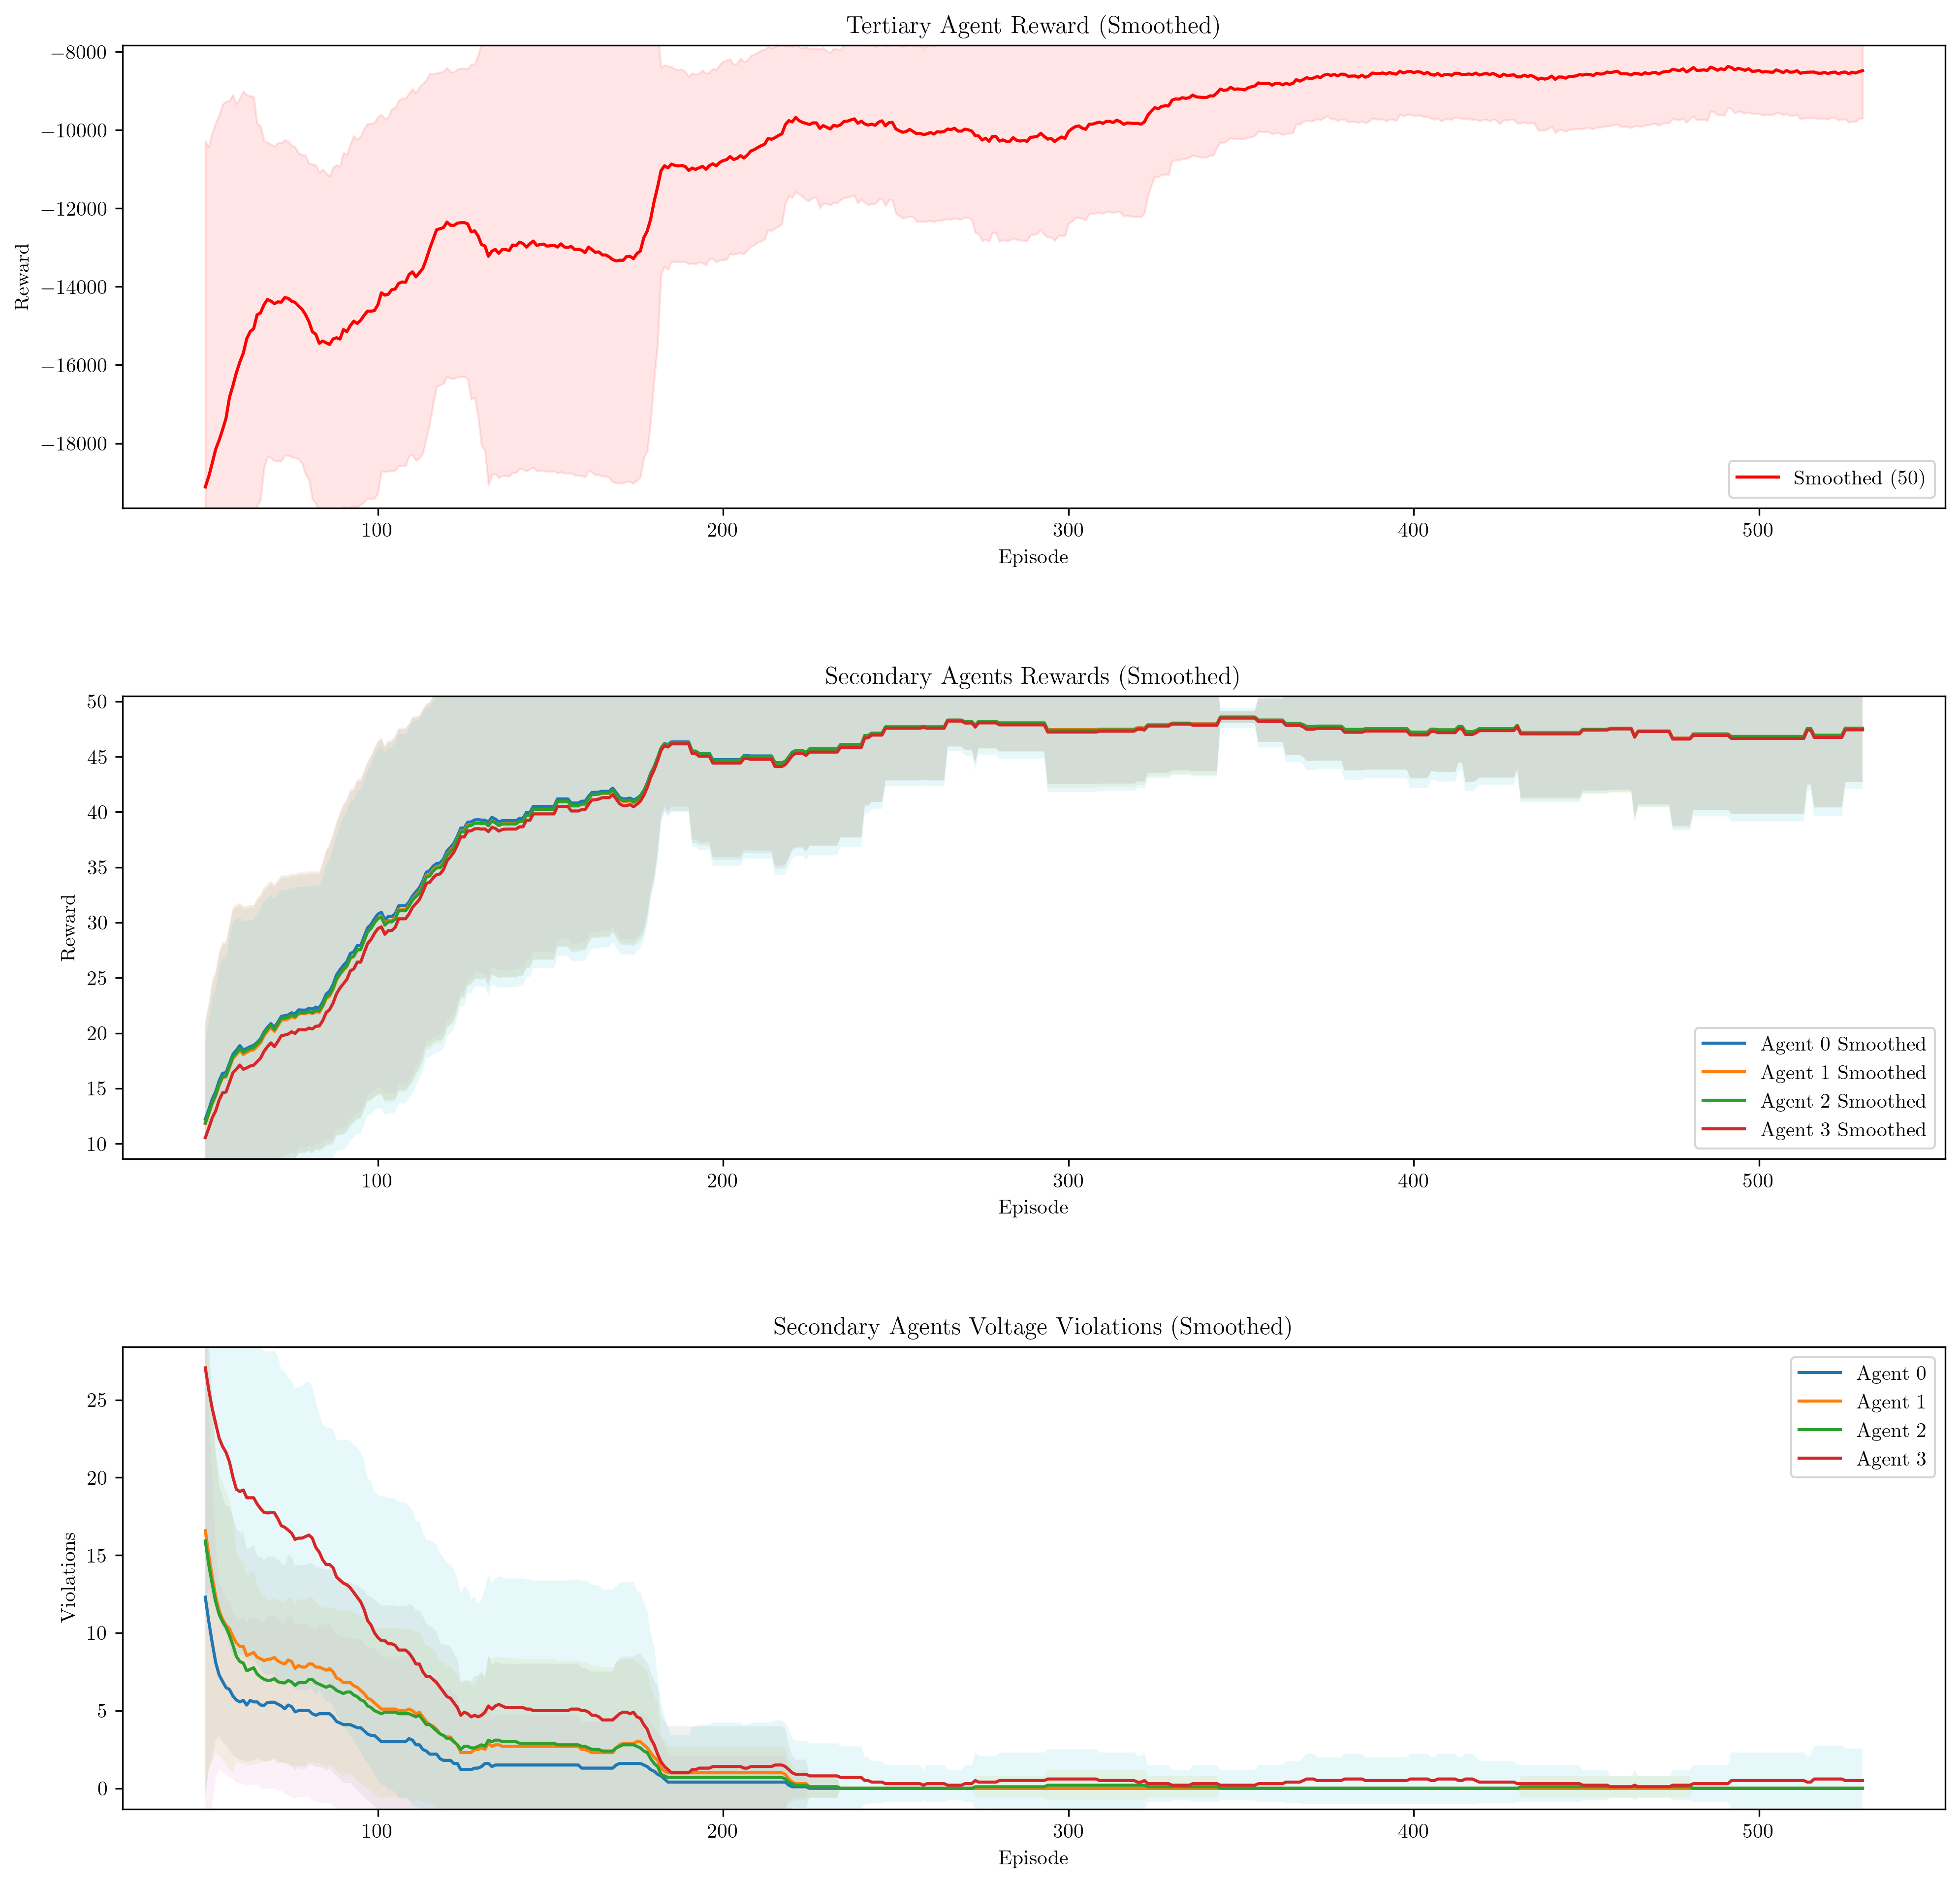
\includegraphics[width=0.9\linewidth]{./rewards_plot.png} 
\captionof{figure}{Convergence of Tertiary and Secondary Agents}
\label{fig:convergence}
\textit{Reward shows convergence of tertiary and secondary agents.}

The reward plot shows the convergence of the tertiary and secondary agents. The reward is calculated as the sum of the rewards of all the agents in the system. The plot shows that the reward converges to a stable value after 500 episodes. The reward is calculated as the sum of the rewards of all the agents in the system. 
The plot shows that the reward converges to a stable value after 500 episodes as shown in Figure \ref{fig:convergence} after which the trend flatlines. The voltage violations of each individual agent is shown in the bottom graph.

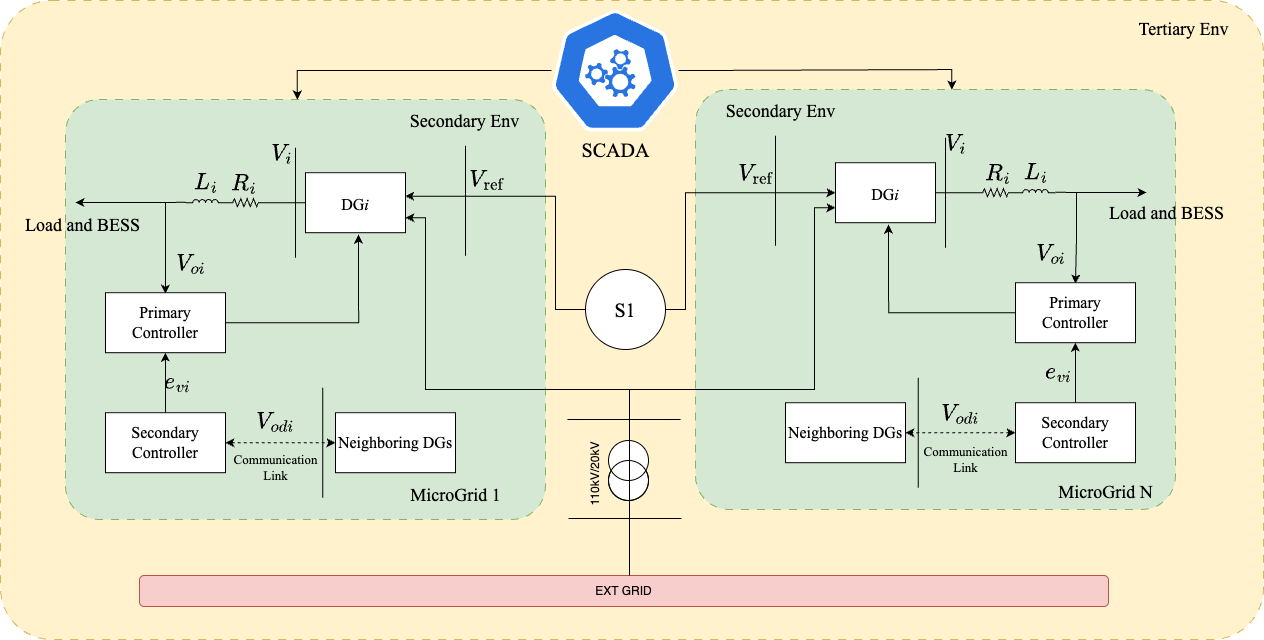
\includegraphics[width=0.9\linewidth]{./der_config.png} 
\captionof{figure}{Electrical diagram showing how two microgrids are connected to the main grid.}
\label{fig:der_config}

\subsection{Future Plots (To be added)}
\begin{itemize}
  \item PV Dispatch vs Grid Power
  \item SOC variation over time
  \item Tie-line energy balance
  \item Voltage profile across buses
\end{itemize}

\section{Conclusion}
The proposed dual-RL architecture offers a robust and scalable approach to hierarchical energy management in fractal microgrids. Preliminary convergence trends are promising. Further analysis will validate system-wide benefits on stability and cost.

\section{GitHub Repository}:
The code for this project is available at \url{https://github.com/vigneshrangaraj/dual-rl-fractal-grid}.

\section*{References}
\begin{itemize}
  \item Apperley, M. (2019). Modelling fractal-structured smart microgrids.
  \item Ji, Y., et al. (2019). Real-time energy management using deep reinforcement learning. \textit{Energies}, 12(12), 2291.
  \item Haarnoja, T., et al. (2018). Soft Actor-Critic Algorithms for Deep RL. arXiv preprint arXiv:1801.01290.
  \item Bidram, A., Davoudi, A., Lewis, F. L., & Qu, Z. (2013). Secondary control of microgrids based on distributed cooperative control of multi‐agent systems. IET Generation, Transmission & Distribution, 7(8), 822-831.
\end{itemize}

\end{document}
